\documentclass[11pt]{article}
\usepackage{listings}
\usepackage{tikz}
%\usepackage{algorithm2e}
\usetikzlibrary{arrows,automata,shapes}
\tikzstyle{block} = [rectangle, draw, fill=blue!20, 
    text width=5em, text centered, rounded corners, minimum height=2em]
\tikzstyle{bt} = [rectangle, draw, fill=blue!20, 
    text width=1em, text centered, rounded corners, minimum height=2em]

\newtheorem{defn}{Definition}
\newtheorem{crit}{Criterion}

\newcommand{\handout}[5]{
  \noindent
  \begin{center}
  \framebox{
    \vbox{
      \hbox to 5.78in { {\bf Software Testing, Quality Assurance and Maintenance } \hfill #2 }
      \vspace{4mm}
      \hbox to 5.78in { {\Large \hfill #5  \hfill} }
      \vspace{2mm}
      \hbox to 5.78in { {\em #3 \hfill #4} }
    }
  }
  \end{center}
  \vspace*{4mm}
}

\newcommand{\lecture}[4]{\handout{#1}{#2}{#3}{#4}{Lecture #1}}
\topmargin 0pt
\advance \topmargin by -\headheight
\advance \topmargin by -\headsep
\textheight 8.9in
\oddsidemargin 0pt
\evensidemargin \oddsidemargin
\marginparwidth 0.5in
\textwidth 6.5in

\parindent 0in
\parskip 1.5ex
%\renewcommand{\baselinestretch}{1.25}

\begin{document}

\lecture{5 --- January 14, 2015}{Winter 2015}{Patrick Lam}{version 0}
\section*{Graph Coverage}

We will discuss graph coverage in great detail. Many forms of software testing
reduce to graph coverage, so once you understand how graph coverage works,
you will have a good understanding of a key software testing topic.

\paragraph{Definition of Graphs.} (You should already be familiar with
this material, but let's establish the terms we'll use in this class). 
Let's start with an example graph.

\begin{minipage}{.4\textwidth}
  \begin{center}
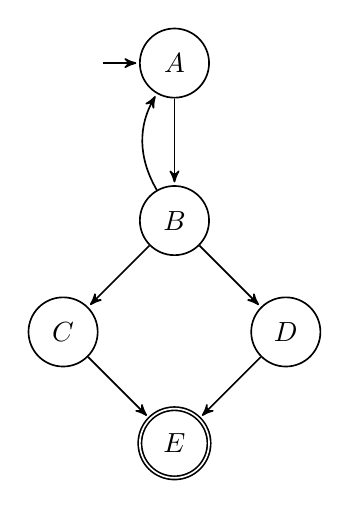
\begin{tikzpicture}[->,>=stealth',shorten >=1pt,auto,node distance=2cm,
                    semithick,initial text=]

  \node[state]         (C)                    {$C$};
  \node[state]         (B) [above right of=C] {$B$};
  \node[initial,state] (A) [above of=B]       {$A$};
  \node[state]         (D) [below right of=B]       {$D$};
  \node[accepting,state]   (E) [below right of=C] {$E$};
  
  \path (A) edge              node {} (B)
        (B) edge [bend left]  node {} (A)
            edge              node {} (C)
            edge              node {} (D)
        (C) edge              node {} (E)
        (D) edge              node {} (E);
\end{tikzpicture}
  \end{center}
\end{minipage} \begin{minipage}{.5\textwidth}
\begin{eqnarray*}
N & : & \mbox{Set of nodes~} \{ A, B, C, D, E \} \\
N_0 & : & \mbox{Set of initial nodes~} \{ A \} \\
N_f & : & \mbox{Set of final nodes~} \{ E \} \\
E \subseteq N \times N & : & \mbox{Edges, e.g. }(A, B)\mbox{ and } (C, E);\\
&& \mbox{~$C$ is the
predecessor and}\\&&\mbox{~~~$E$ is the successor in $(C, E)$.}
\end{eqnarray*}
\end{minipage}

\newcommand{\Ns}{\ensuremath{N_{\mbox{\scriptsize sub}}}}

\paragraph{Subgraph:} Let $G'$ be a subgraph of $G$; 
then the nodes of $G'$ must be a subset $\Ns$ of $N$.
Then the initial nodes of $G'$ are $N_0 \cap \Ns$ and its final nodes
are $N_f \cap \Ns$. The edges of $G'$ are $E \cap (\Ns \times
\Ns)$. 

For example, consider the case where we set $\Ns = \{ A, B, E \}$.
This induces the subgraph:

\begin{center}
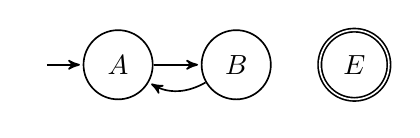
\begin{tikzpicture}[->,>=stealth',shorten >=1pt,auto,node distance=1.5cm,
                    semithick,initial text=]

  \node[initial,state]   (A)        {$A$};
  \node[state]           (B) [right of=A] {$B$};
  \node[accepting,state] (E) [right of=B] {$E$};
  
  \path (A) edge              node {} (B);
  \path (B) edge [bend left]  node {} (A);
\end{tikzpicture}
\end{center}
Note that graphs need not be connected.

\paragraph{Paths.} The most important thing about a graph, for testing
purposes, is the path through the graph. Here is a graph $G_\#$ and some example
paths through the graph.

\begin{center}
\begin{tikzpicture}[->,>=stealth',shorten >=1pt,auto,node distance=2.8cm,
                    semithick,initial text=]

  \node[initial,state]   (1)              {$1$};
  \node[state]           (2) [right of=1] {$2$};
  \node[state]           (3) [right of=2] {$3$};
  \node[state]           (4) [above of=3] {$4$};
  \node[state]           (5) [right of=3] {$5$};
  \node[state]           (6) [right of=5] {$6$};
  \node[accepting,state] (7) [right of=6] {$7$};
  
  \path (1) edge              node {} (2)
        (2) edge              node {} (3)
            edge              node {} (4)
        (3) edge              node {} (5)
        (4) edge              node {} (5)
        (5) edge              node {} (6)
        (6) edge              node {} (7)
            edge [bend left]  node {} (2);
\end{tikzpicture}
\end{center}

\begin{itemize}
\item path 1: $[2, 3, 5]$, with length $2$.
\item path 2: $[1, 2, 3, 5, 6, 2]$, with length $5$.
\item not a path: $[1, 2, 5]$.
\end{itemize}

We say that path 1 is \emph{from} node 2 \emph{to} node 5. We
can also say that path 1 is \emph{from} edge $(2, 3)$ \emph{to} 
$(3, 5)$.

\begin{defn} 
A \emph{path} is a sequence of nodes from a graph $G$ whose 
adjacent pairs all belong to the set of edges $E$ of $G$.
\end{defn}

Note that length 0 paths are still paths.

\begin{defn} 
A \emph{subpath} is a subsequence of a path.
\end{defn}
This textbook definition is ambiguous: is $[1,2,5]$ a subpath of
$[1,2,3,5,6,2]$?

\begin{defn} 
  A \emph{subsequence} is a sequence that can be derived from another
  sequence by deleting some elements without changing the order of the
  remaining elements.
\end{defn}
Yes, $[1,2,5]$ is a subsequence of $[1,2,3,5,6,2]$. However, $[1,2,5]$ is not a
path, so we are going to say that it is not a subpath.

\subsection*{Test cases and test paths.} Some paths are also test paths.
Here is a test path from
$G_\#$: 
\[ [1, 2, 3, 5, 6, 7]; \]
here is another one:
\[ [1, 2, 3, 5, 6, 2, 3, 5, 6, 7]. \]
You can easily come up with more paths. Now, test paths are linked to
test cases. First, let's define the notion of a test path.

\begin{defn} A \emph{test path} is a path $p$ (possibly of length 0)
that starts at some node in $N_0$ and ends at some node in $N_f$.
\end{defn}

Running the test case on the program or method yields one or more test
paths. A test path may represent many test cases (for instance, if a
program takes the same branches on all of those test cases); or a 
test path may represent no test cases (if it is infeasible).

\paragraph{Paths and semantics.} When a graph is a program's control-flow
graph, some of the paths in the graph may not correspond to program
semantics. Consider the following graph.

\tikzstyle{decision} = [diamond, draw, fill=blue!20, 
    text width=4.4em, text ragged, node distance=3cm, inner sep=0pt]
\tikzstyle{block} = [rectangle, draw, fill=blue!20, 
    text width=3em, text centered, rounded corners, minimum height=2em]

\begin{center}
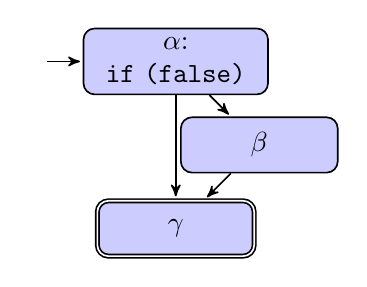
\begin{tikzpicture}[->,>=stealth',shorten >=1pt,auto,node distance=1.5cm,
                    semithick,initial text=]

  \node[initial,block,text width=6em]   (A)              {$\alpha$: \mbox{\tt if (false)}};
  \node[block]           (B) [below right of=A] {$\beta$};
  \node[accepting,block] (C) [below left of=B] {$\gamma$};
  
  \path (A) edge              node {} (B)
        (A) edge              node {} (C)
        (B) edge              node {} (C);
\end{tikzpicture}
\end{center}
Clearly $\beta$ will never execute. 

In this course, we will generally only talk about the \emph{syntax} of a graph---its nodes
and edges---and not its \emph{semantics}.

However, in the following definition, we'll talk about both notions.
\begin{defn}
A node $n$ (or edge $e$) is \emph{syntactically reachable} from $n_i$
if there exists a path from $n_i$ to $n$ (or $e$). A node $n$ (or edge $e$)
is \emph{semantically reachable} if one of the paths from $n_i$ to $n$
can be reached on some input.
\end{defn}

Standard graph algorithms, like breadth-first search and depth-first
search, can compute syntactic reachability. (Semantic reachability is
undecidable; no algorithm can precisely compute semantic reachability
for all programs.)

We define $\mbox{reach}_G(\chi)$ as the portion of the graph syntactically reachable
from $\chi$. ($\chi$ might be a node, an edge, a set of nodes, or a set
of edges.) For example:
\begin{itemize}
\item $\mbox{reach}_G(N_0)$ is the set of nodes and edges reachable from
the initial node(s);
\item $\mbox{reach}_{G\#}(2)$ in the above graph $G_\#$ is $\{2, 3, 4, 5, 6, 7\}$;
\item $\mbox{reach}_{G\#}(7)$ is $\{7\}$.
\end{itemize}
Note that we include $\chi$ in the set of nodes reachable from $\chi$, because
paths of length 0 are paths.

When we talk about the nodes or edges in a graph $G$ in a coverage
criterion, we'll generally mean $\mbox{reach}_G(N_0)$; the unreachable nodes
tend to (1) be uninteresting; and (2) to frustrate coverage criteria.



\end{document}

